This chapter documents the prototyping phase of the UrbanPulse platform, covering
the technology selection rationale, containerised infrastructure design, core data
schema decisions, and the incremental validation strategy used before full
implementation began.

% ============================================================
\section{Technology Stack Selection}
\label{sec:tech-selection}
% ============================================================

The UrbanPulse prototype is built on a curated stack of open-source components.
Each technology was evaluated against three criteria: \textit{(i)} compatibility
with Python 3.12 and the \texttt{uv} monorepo toolchain, \textit{(ii)} support
for streaming-first workloads, and \textit{(iii)} availability as a
self-hostable Docker image suitable for homelab deployment.
Table~\ref{tab:tech-stack} summarises the chosen components and their roles.

\begin{table}[htbp]
\centering
\caption{UrbanPulse technology stack and selection rationale.}
\label{tab:tech-stack}
\resizebox{\textwidth}{!}{%
\begin{tabular}{llll}
\hline
\textbf{Component} & \textbf{Technology} & \textbf{Version} & \textbf{Rationale} \\
\hline
Message Broker     & Redpanda            & v25.3.10 & Kafka-compatible; no ZooKeeper; lower memory \\
Object Storage     & MinIO               & latest   & S3-compatible API; local deployment \\
Table Format       & Apache Iceberg      & 0.9.x    & Schema evolution; time-travel; partition pruning \\
Catalog            & Project Nessie      & 0.99.0   & Git-like branching; REST API \\
Online Store       & PostgreSQL          & 15       & UPSERT semantics; asyncpg for async serving \\
Vector Store       & ChromaDB            & 0.4.x    & Embedded; nomic-embed compatible \\
Orchestration      & Prefect             & 3.x      & Task retries; flow scheduling; UI dashboard \\
ML Tracking        & MLflow              & 2.21.3   & Experiment logging; model registry \\
LLM Runtime        & Ollama              & latest   & Local GPU inference; Qwen2.5:3b \\
Serving            & FastAPI             & 0.115.x  & Async; SSE support; Pydantic v2 \\
Reverse Proxy      & Traefik             & v3       & Automatic TLS; label-based routing \\
Monitoring         & Grafana + Loki      & latest   & Log aggregation; dashboard \\
Frontend           & Next.js 15 + TypeScript & 15   & App Router; real-time SSE client \\
\hline
\end{tabular}%
}
\end{table}

\subsection{Message Broker: Redpanda over Apache Kafka}

\textbf{Redpanda}~\cite{redpanda_whitepaper} was selected over vanilla Apache
Kafka for two practical reasons. First, Redpanda eliminates the ZooKeeper
dependency, reducing the container count by two services. Second, its
\textit{single-binary} architecture yields lower memory consumption, which
is critical for the homelab Intel~i5 deployment environment. The Kafka-wire
compatibility ensures that all \texttt{confluent\_kafka} Python clients work
without modification.

\subsection{Storage: Iceberg + Nessie + MinIO}

Raw Parquet files in MinIO constitute the \textbf{Bronze layer}. Promoting
data to \textbf{Silver} and \textbf{Gold} requires a table format that
supports (a) transactional writes from micro-batches, (b) schema evolution
without full rewrites, and (c) time-travel for reprocessing. \textbf{Apache
Iceberg}~\cite{iceberg_paper} satisfies all three. \textbf{Project
Nessie}~\cite{nessie_docs} provides the REST catalog, enabling branching and
atomic commits without locking MinIO objects directly.

\subsection{LLM: Ollama with Qwen2.5:3b}

The RAG pipeline requires a model that fits within the homelab GPU budget
(NVIDIA GTX~1060, 6~GB VRAM). \textbf{Qwen2.5:3b}~\cite{qwen25_report},
served via \textbf{Ollama}, achieves an average time-to-first-token of under
one second while producing coherent 2--3 sentence traffic explanations in
both English and Vietnamese. The \textit{RAG-over-fine-tuning} approach is
justified by the need for always-current context: retraining on new anomaly
events would be prohibitively expensive on the available hardware.

% ============================================================
\section{Service Topology Design}
\label{sec:topology}
% ============================================================

The platform is decomposed into \textbf{six microservices}, each running as an
independent Docker container. Services communicate exclusively through two
channels: the \textbf{Redpanda broker} (event streams) and
\textbf{PostgreSQL} (materialised feature store). No direct service-to-service
HTTP calls exist in the hot path, ensuring fault isolation.

Figure~\ref{fig:service-topology} illustrates the container topology and the
two communication channels.

\begin{figure}[htbp]
\centering
\resizebox{0.92\textwidth}{!}{%
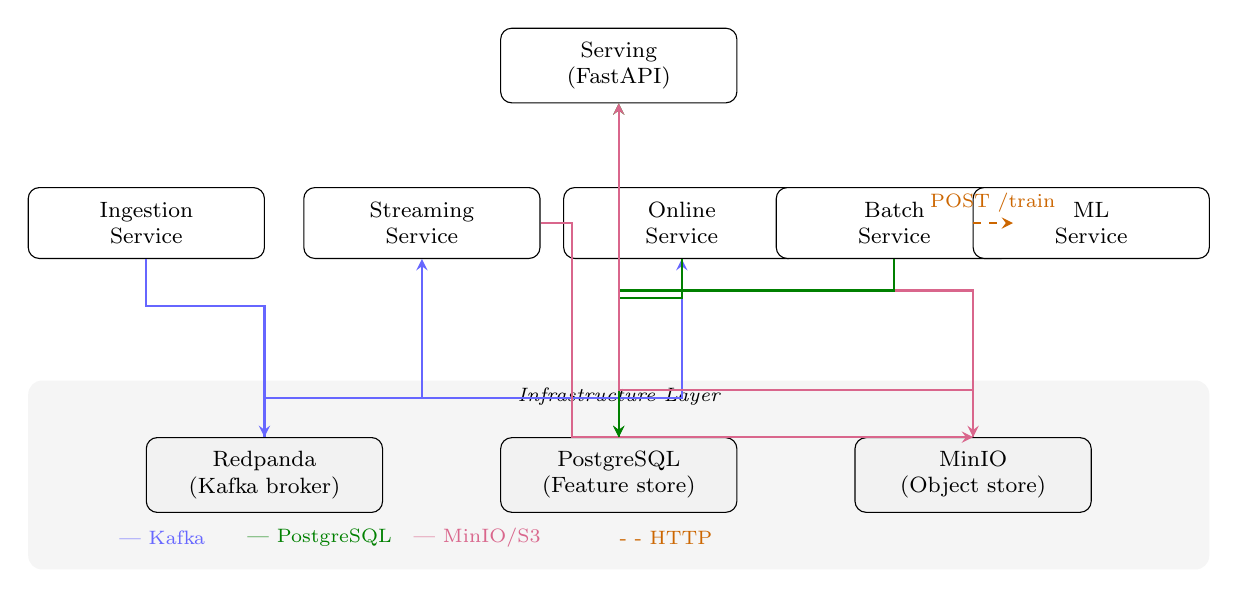
\begin{tikzpicture}[
  >=stealth, font=\small,
  svc/.style={draw, rounded corners=4pt, fill=white,
              minimum width=3.0cm, minimum height=0.9cm,
              align=center, font=\footnotesize, inner sep=5pt},
  infra/.style={draw, rounded corners=4pt, fill=gray!10,
                minimum width=3.0cm, minimum height=0.9cm,
                align=center, font=\footnotesize, inner sep=5pt},
  karr/.style={->, thick, blue!60},
  parr/.style={->, thick, green!50!black},
  harr/.style={->, thick, orange!80!black},
  lbl/.style={font=\scriptsize}
]

%% Infrastructure layer (bottom band)
\fill[gray!8, rounded corners=5pt] (-7.5,-1.2) rectangle (7.5,1.2);
\node[font=\scriptsize\itshape] at (0,1.0) {Infrastructure Layer};
\node[infra] (redpanda) at (-4.5, 0) {Redpanda\\(Kafka broker)};
\node[infra] (postgres) at (0,    0) {PostgreSQL\\(Feature store)};
\node[infra] (minio)    at (4.5,  0) {MinIO\\(Object store)};

%% Application services (top)
\node[svc] (ingest)    at (-6.0,  3.2) {Ingestion\\Service};
\node[svc] (streaming) at (-2.5,  3.2) {Streaming\\Service};
\node[svc] (online)    at ( 0.8,  3.2) {Online\\Service};
\node[svc] (batch)     at ( 3.5,  3.2) {Batch\\Service};
\node[svc] (ml)        at ( 6.0,  3.2) {ML\\Service};
\node[svc] (serving)   at ( 0.0,  5.2) {Serving\\(FastAPI)};

%% Ingest → Redpanda
\draw[karr] (ingest.south) -- ++(0,-0.6) -| (redpanda.north);

%% Redpanda → Streaming, Online
\draw[karr] (redpanda.north) -- ++(0,0.5) -| (streaming.south);
\draw[karr] (redpanda.north) -- ++(0,0.5) -| (online.south);

%% Streaming → MinIO
\draw[->, thick, purple!60] (streaming.east) -- ++(0.4,0) |- (minio.north);

%% Online → PostgreSQL
\draw[parr] (online.south) -- ++(0,-0.5) -| (postgres.north);

%% Batch → MinIO (read/write) + PostgreSQL (write baseline)
\draw[->, thick, purple!60] (batch.south) -- ++(0,-0.4) -| (minio.north);
\draw[parr] (batch.south)   -- ++(0,-0.4) -| (postgres.north);

%% ML ↔ MLflow (external, simplified as arrow to batch)
\draw[harr, dashed] (ml.west) -- (batch.east) node[midway, above, lbl] {POST /train};

%% Serving ← PostgreSQL + MinIO
\draw[parr] (postgres.north) -- ++(0,1.0) -| (serving.south);
\draw[->, thick, purple!60] (minio.north) -- ++(0,0.6) -| (serving.south);

%% Legend
\node[lbl, blue!60]            at (-5.8,-0.8)  {--- Kafka};
\node[lbl, green!50!black]     at (-3.8,-0.8)  {--- PostgreSQL};
\node[lbl, purple!60]          at (-1.8,-0.8)  {--- MinIO/S3};
\node[lbl, orange!80!black]    at ( 0.6,-0.8)  {- - HTTP};

\end{tikzpicture}%
}
\caption{UrbanPulse service topology: six microservices communicating via
         Redpanda (blue) and PostgreSQL (green). Dashed orange indicates the
         HTTP trigger from Batch to ML service.}
\label{fig:service-topology}
\end{figure}

% ============================================================
\section{Data Schema Design}
\label{sec:schema-design}
% ============================================================

\subsection{Kafka Message Schema}

Every traffic observation published to Redpanda is serialised as JSON conforming
to the \texttt{TrafficRouteObservation} Pydantic model. The canonical fields are:

\begin{itemize}
  \item \textbf{\texttt{route\_id}}: unique string identifier of the inter-zone
        route (e.g., \texttt{zone1\_urban\_core\_\allowbreak to\_zone2\_eastern\_innovation}).
  \item \textbf{\texttt{duration\_ms}}: raw travel time from the VietMap Directions
        API, in milliseconds.
  \item \textbf{\texttt{duration\_minutes}}: derived field ($= \texttt{duration\_ms}
        / 60000$), rounded to one decimal place.
  \item \textbf{\texttt{congestion}}: nested object containing
        \texttt{heavy\_ratio}, \texttt{moderate\_ratio},
        \texttt{low\_ratio} (each a fraction $[0,1]$),
        \texttt{severe\_segments} (integer count), and
        \texttt{total\_segments}.
  \item \textbf{\texttt{timestamp\_utc}}: ISO-8601 timestamp at which the API
        was polled.
\end{itemize}

\noindent A Kafka header \texttt{ingest\_ts} (Unix milliseconds) is attached at
publish time to enable end-to-end ingestion lag measurement in the Online Service.

\subsection{Iceberg Table Schemas}

Three Iceberg tables are provisioned in MinIO via Nessie catalog:

\begin{enumerate}
  \item \textbf{Silver} (\texttt{silver.traffic\_route}): 13-column schema
        with one row per API observation. Partitioned by \texttt{day(timestamp\_utc)}.
        A \texttt{source} column records the VietMap API endpoint version.
  \item \textbf{Gold} (\texttt{gold.traffic\_hourly}): 11-column hourly
        aggregation keyed by \texttt{(route\_id, hour\_utc)}. Includes
        \texttt{avg\_heavy\_ratio}, \texttt{avg\_moderate\_ratio},
        \texttt{avg\_duration\_minutes}, and \texttt{p95\_duration\_minutes}.
        Partitioned by \texttt{day(hour\_utc)}.
  \item \textbf{Baseline} (\texttt{gold.traffic\_baseline}): per-route,
        per-hour-of-day, per-day-of-week statistical summary used by the
        Online Service Z-score computation.
\end{enumerate}

\subsection{PostgreSQL Online Store}

The table \texttt{online\_route\_features} persists the current hourly window
state for every route, with primary key \texttt{(route\_id, window\_start)}.
It serves two purposes: (a) it is the low-latency read target of the Serving
API, and (b) it acts as a crash-recovery checkpoint --- on restart, the Online
Service reconstructs Welford accumulators from stored
\texttt{mean} and \texttt{stddev} values via the identity
$M_2 = \sigma^2 \times (n - 1)$.

% ============================================================
\section{Infrastructure Prototyping}
\label{sec:infra-proto}
% ============================================================

The entire platform is containerised using \textbf{Docker Compose} with a
three-file layered override pattern:

\begin{itemize}
  \item \texttt{docker-compose\allowbreak.base.yaml} --- shared service definitions
        (Redpanda, MinIO, Nessie, PostgreSQL, ChromaDB, MLflow, Prefect, Ollama).
  \item \texttt{docker-compose\allowbreak.dev.yaml} --- development overlay: exposes ports
        locally, mounts source code volumes, uses \texttt{host.docker.internal}
        for the Ollama endpoint.
  \item \texttt{docker-compose\allowbreak.prod.yaml} --- production overlay: adds
        Traefik reverse proxy with Let's Encrypt TLS, removes exposed ports,
        uses named volumes at \texttt{/opt/urban-pulse/} on the host.
\end{itemize}

\noindent The \texttt{Makefile} provides validated entry points (\texttt{make dev},
\texttt{make prod}, \texttt{make bootstrap}, \texttt{make train}) so that the
multi-container stack can be brought up or torn down deterministically. The
\texttt{bootstrap} target seeds Redpanda topics, MinIO buckets, and Prefect
deployment schedules in a single pass before live traffic is processed.
